\chapter{Unsupervised Clustering for Spatial Homogenization}
\label{chap:unsupervised}

first paragraph: motivation
-recall from previous chapter:
  -found clusters in \ac{MGXS}
  -must cluster \ac{MGXS} to reduce U-238 capture rate errors to level of fission
-motivate chapter two-fold:
  -simultaneously achieve degenerate's accuracy and null's convergence
  -KEY: need to be more adapative than \ac{LNS} for arbitrary geometries

second paragraph: over-arching goal
-achieve accuracy of \ac{MC} with efficient deterministic multi-group methods
-recall motivation in chapter 1??
-present flow chart figure Fig.~\ref{fig:chap10-flow-chart}
-following chapter will evaluate methodology wrt eigenvalues, fission rates, U-238 capture reats

third paragraph: outline chapter
-Sec.~\ref{}

-need to say that chapter presents a general methodology, only part of which will be evaluated in the following chapter

\begin{figure}
  \centering
  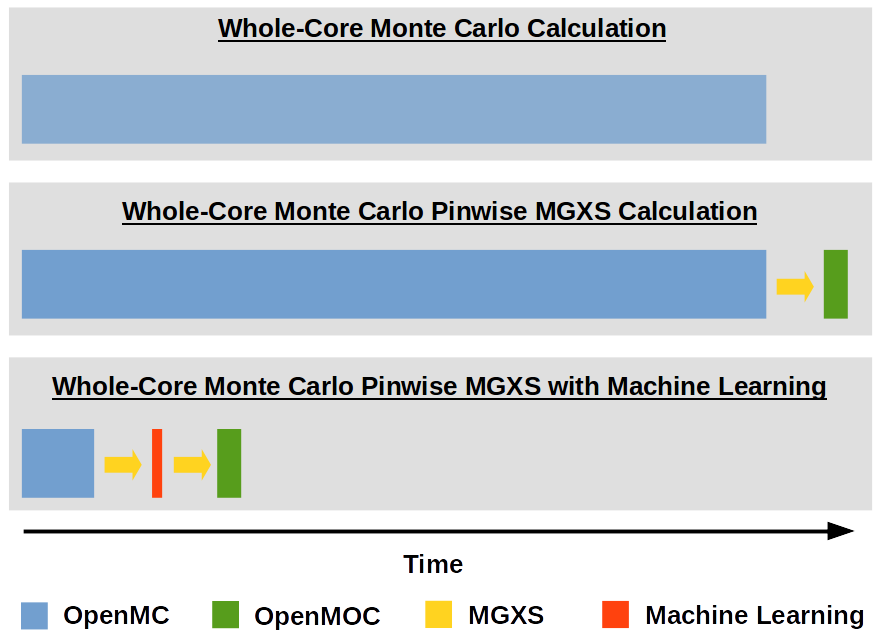
\includegraphics[width=0.9\linewidth]{figures/unsupervised/flow-chart}
  \caption{}
\caption[flowchar]{flowchart}
\label{fig:chap10-flow-chart}
\end{figure}
  

%%%%%%%%%%%%%%%%%%%%%%%%%%%%%%%%%%%%%%%%%%%%%%%%%%%%%%%%%%%%%%%%%%%%%%%%%%%%%%%
\section{Latent Spectral Index Model}
\label{sec:chap10-latent-model}

-\ac{LSIM} - latent variable model
-three goals:
  -infer number of points/pins in each set
  -infer conditional probabilities?
  -assign each region to the most likely set?
-is this section needed???


%%%%%%%%%%%%%%%%%%%%%%%%%%%%%%%%%%%%%%%%%%%%%%%%%%%%%%%%%%%%%%%%%%%%%%%%%%%%%%%
\section{Overview of Approach}
\label{sec:chap10-overview}

-competing paragidms:
  -clustering
  -input -> target (e.g., trees)
  -some combination of the two

-break apart diagram for machine learning piece into parts
  -clustering
    -flow chart: litmus tests, feature eng./selectiontransformation, clustering
  -input -> target (e.g., regression)
    -flow chart: litmus tests, target selection, feature eng./selection/transformation, model fitting, prediction
     -can take outputs as inputs for clustering scheme


%%%%%%%%%%%%%%%%%%%%%%%%%%%%%%%%%%%%%%%%%%%%%%%%%%%%%%%%%%%%%%%%%%%%%%%%%%%%%%%
\section{Feature Engineering}
\label{sec:chap10-feature-engineer}

first paragraph: motivation
-need to define ``feature''
-recall plots from preceding chapter with clusters
-identify features which are only derived from tallied quantities
-mention conflict:
  -need 70+ groups for accurate solutions
  -uncertainties / noise in few-group \ac{MGXS} is less, making it easier to identify clusters
-cluster \ac{MGXS} directly
  -simply draw 1D boundaries b/w \ac{MGXS} in histograms
  -could cluster multiple microscopic \ac{MGXS} simultaneously - nuclides, reactions, groups
  -multiple \ac{MGXS} may eliminate ``de-noise'' data, eliminate outliers
    -good segue to next paragraph!!

second paragraph: more generally
-include non-\ac{MGXS} variables to cluster
  -separation distance clusters may grow with more variables, making them easier to identify
-goal: identify variables which reflect spatial self-shielding effects
-can simply cluster multiple micro \ac{MGXS} simultaneously

third paragraph: outline
-

-mention that some features may be 1) fuel pin specific (at the least), 2) nuclide specific, 3) reaction specific, 4) energy group specific

%%%%%%%%%%%%%%%%%%%%%%%%%%%%%%%%%%%%
\subsection{Statistical Uncertainty}
\label{subsec:chap10-stat-uncertainty}

first paragraph: explain what it is
-point to a few figures
-explain why std. dev. may be higher for different pins
-indicate that it may reflect the difference in track density in differen pins
  -is this why we see rings in the \ac{MGXS} in the full core??
-recall equation for std. dev.
-recall uncertainty propagation
-also relative error - normalize out the mean \ac{MGXS}

-MATCH COLOR SCHEMES

\begin{equation}
\label{eqn:chap10-rel-err}
\eta_{x,i,k,g} = \frac{\sigma_{\hat{\sigma}_{x,i,k,g}}}{\hat{\sigma}_{x,i,k,g}}
\end{equation}

second paragraph: visualizations
-look at single fuel assembly with GUI
-three plots: full, two different clusters selected

\begin{figure}[h!]
\centering
\begin{subfigure}{0.42\textwidth}
  \centering
  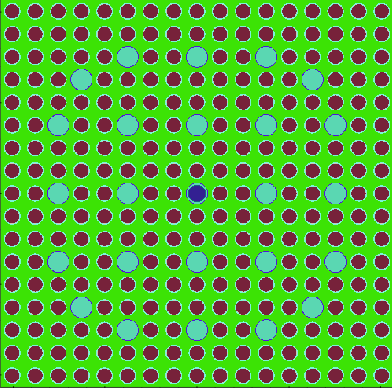
\includegraphics[width=0.9\linewidth]{figures/unsupervised/features/assm-16/geometry}
  \caption{}
  \label{fig:chap10-fiss-mean-std-geom}
\end{subfigure}%
\begin{subfigure}{0.42\textwidth}
  \centering
  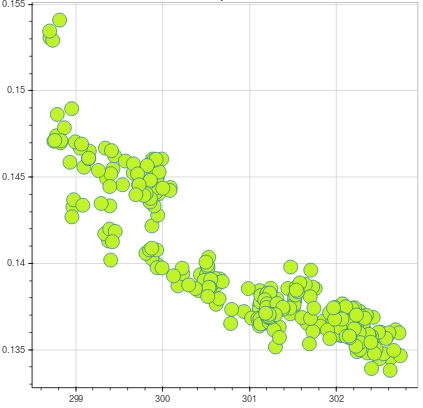
\includegraphics[width=0.9\linewidth]{figures/unsupervised/features/assm-16/u235-fiss/mean-std/mgxs}
  \caption{}
  \label{fig:chap10-fiss-mean-std-mgxs}
\end{subfigure}
\begin{subfigure}{0.42\textwidth}
  \centering
  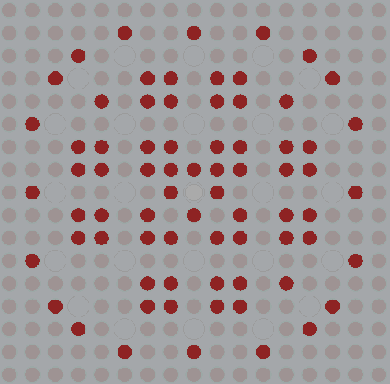
\includegraphics[width=0.9\linewidth]{figures/unsupervised/features/assm-16/u235-fiss/mean-std/geometry-2}
  \caption{}
  \label{fig:chap10-fiss-mean-std-geom-2}
\end{subfigure}%
\begin{subfigure}{0.42\textwidth}
  \centering
  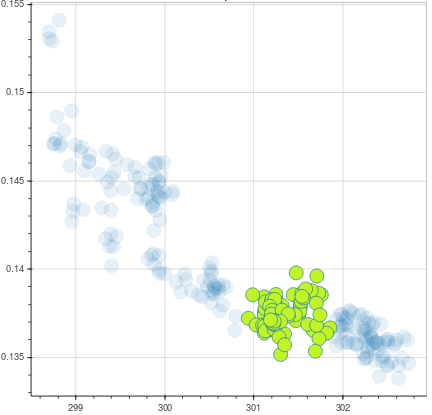
\includegraphics[width=0.9\linewidth]{figures/unsupervised/features/assm-16/u235-fiss/mean-std/mgxs-2}
  \caption{}
  \label{fig:chap10-fiss-mean-std-mgxs-2}
\end{subfigure}
\begin{subfigure}{0.42\textwidth}
  \centering
  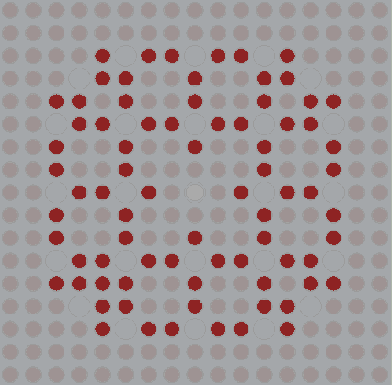
\includegraphics[width=0.9\linewidth]{figures/unsupervised/features/assm-16/u235-fiss/mean-std/geometry-3}
  \caption{}
  \label{fig:chap10-fiss-mean-std-geom-3}
\end{subfigure}%
\begin{subfigure}{0.42\textwidth}
  \centering
  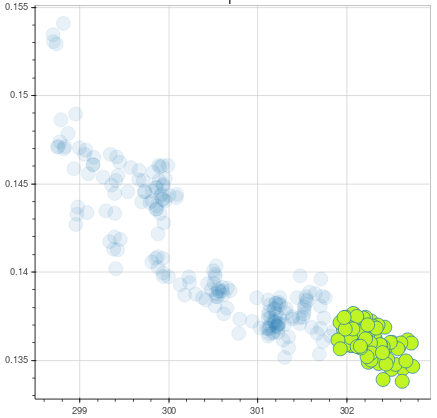
\includegraphics[width=0.9\linewidth]{figures/unsupervised/features/assm-16/u235-fiss/mean-std/mgxs-3}
  \caption{}
  \label{fig:chap10-fiss-mean-std-mgxs-3}
\end{subfigure}
\caption[Clustering of U-235 fission MGXS standard deviations]{Scatter plots of the pin-wise U-235 fission (group 2 of 2) \ac{MGXS} means ($x$) and standard deviations ($y$) for the 1.6\% enriched fuel assembly.}
\label{fig:chap10-mean-std}
\end{figure}

\clearpage

\begin{figure}[h!]
\centering
\begin{subfigure}{0.42\textwidth}
  \centering
  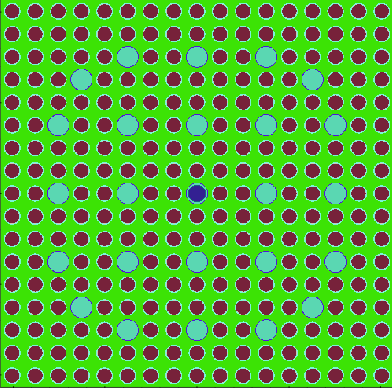
\includegraphics[width=0.9\linewidth]{figures/unsupervised/features/assm-16/geometry}
  \caption{}
  \label{fig:chap10-capt-mean-std-geom}
\end{subfigure}%
\begin{subfigure}{0.42\textwidth}
  \centering
  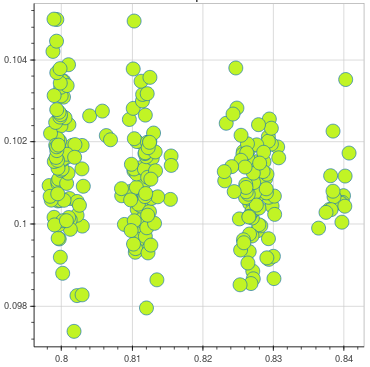
\includegraphics[width=0.9\linewidth]{figures/unsupervised/features/assm-16/u238-capt/mean-std/mgxs}
  \caption{}
  \label{fig:chap10-capt-mean-std-mgxs}
\end{subfigure}
\begin{subfigure}{0.42\textwidth}
  \centering
  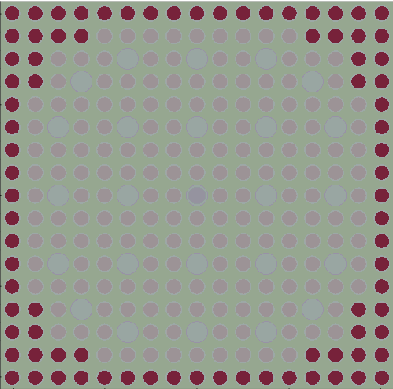
\includegraphics[width=0.9\linewidth]{figures/unsupervised/features/assm-16/u238-capt/mean-std/geometry-2}
  \caption{}
  \label{fig:chap10-capt-mean-std-geom-2}
\end{subfigure}%
\begin{subfigure}{0.42\textwidth}
  \centering
  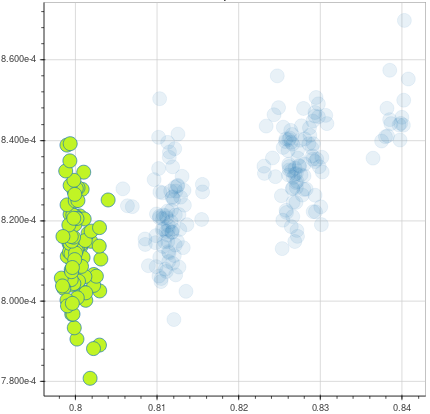
\includegraphics[width=0.9\linewidth]{figures/unsupervised/features/assm-16/u238-capt/mean-std/mgxs-2}
  \caption{}
  \label{fig:chap10-capt-mean-std-mgxs-2}
\end{subfigure}
\begin{subfigure}{0.42\textwidth}
  \centering
  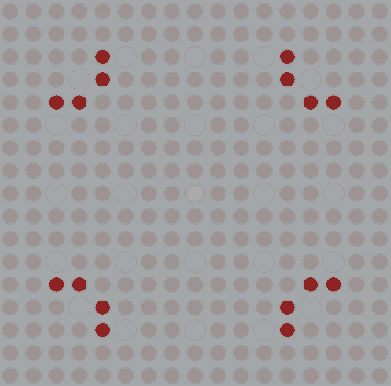
\includegraphics[width=0.9\linewidth]{figures/unsupervised/features/assm-16/u238-capt/mean-std/geometry-3}
  \caption{}
  \label{fig:chap10-capt-mean-std-geom-3}
\end{subfigure}%
\begin{subfigure}{0.42\textwidth}
  \centering
  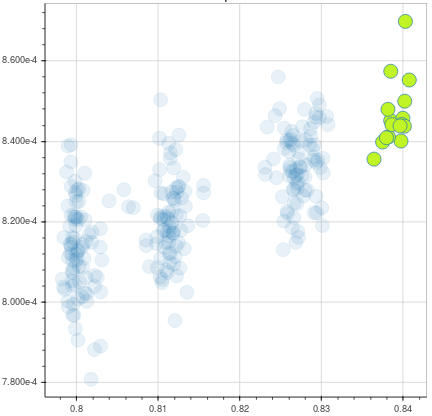
\includegraphics[width=0.9\linewidth]{figures/unsupervised/features/assm-16/u238-capt/mean-std/mgxs-3}
  \caption{}
  \label{fig:chap10-capt-mean-std-mgxs-3}
\end{subfigure}
\caption[Clustering of U-238 capture MGXS standard deviations]{Scatter plots of the pin-wise U-238 capture (group 1 of 2) \ac{MGXS} means ($x$) and standard deviations ($y$) for the 1.6\% enriched fuel assembly.}
\label{fig:chap10-mean-std}
\end{figure}

\clearpage

%%%%%%%%%%%%%%%%%%%%%%%%%%%%%%%%%%
\subsection{Fractional Reactivity}
\label{subsec:chap10-frac-reactivity}

first paragraph: explain what it is
-divide each pin's energy-integrated nu-fission rxn rate by the total energy- and volume-integrated absorption rates across all fuel pins
-Eqn.~\ref{eqn:chap10-frac-reactivity}
  -multiply by 1E5 to get units of \ac{pcm}
-explain what it indicates (differential moderation, adjacency to guide tubes, spectral hardening)
-note that $k$ is ONLY for fuel regions!!!

\begin{equation}
\label{eqn:chap10-frac-reactivity}
\alpha_{k} = \frac{\displaystyle\sum\limits_{g=1}^{G}\nu\hat{\sigma}_{f,i,k,g}\hat{\phi}_{k,g}}{\displaystyle\sum\limits_{k=1}^{K}\displaystyle\sum\limits_{g=1}^{G}\hat{\sigma}_{a,i,k,g}\hat{\phi}_{k,g}}
\end{equation}

second paragraph: visualizations
-look at single fuel assembly with GUI
-three plots: full, two different clusters selected

\begin{figure}[h!]
\centering
\begin{subfigure}{0.45\textwidth}
  \centering
  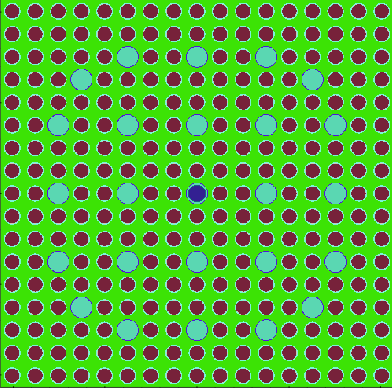
\includegraphics[width=0.9\linewidth]{figures/unsupervised/features/assm-16/geometry}
  \caption{}
  \label{fig:chap10-fiss-mean-pcm-geom}
\end{subfigure}%
\begin{subfigure}{0.45\textwidth}
  \centering
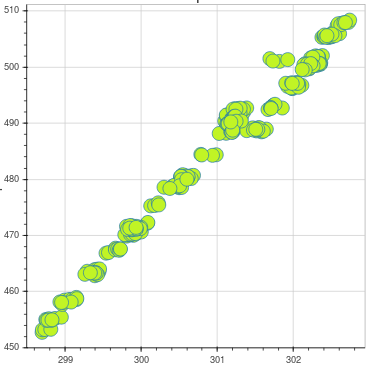
\includegraphics[width=0.9\linewidth]{figures/unsupervised/features/assm-16/u235-fiss/mean-pcm/mgxs}
  \caption{}
  \label{fig:chap10-fiss-mean-pcm-mgxs}
\end{subfigure}
\begin{subfigure}{0.45\textwidth}
  \centering
  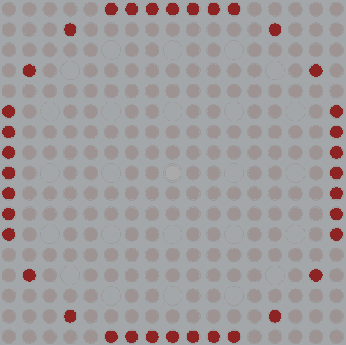
\includegraphics[width=0.9\linewidth]{figures/unsupervised/features/assm-16/u235-fiss/mean-pcm/geometry-2}
  \caption{}
  \label{fig:chap10-fiss-mean-pcm-geom-2}
\end{subfigure}%
\begin{subfigure}{0.45\textwidth}
  \centering
  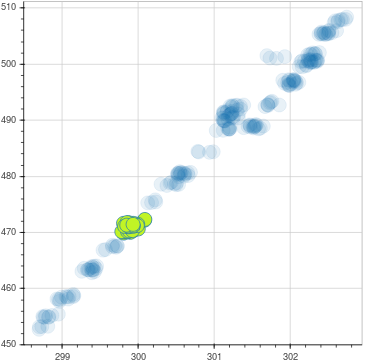
\includegraphics[width=0.9\linewidth]{figures/unsupervised/features/assm-16/u235-fiss/mean-pcm/mgxs-2}
  \caption{}
  \label{fig:chap10-fiss-mean-pcm-mgxs-2}
\end{subfigure}
\begin{subfigure}{0.45\textwidth}
  \centering
  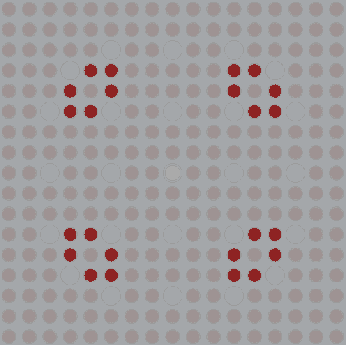
\includegraphics[width=0.9\linewidth]{figures/unsupervised/features/assm-16/u235-fiss/mean-pcm/geometry-3}
  \caption{}
  \label{fig:chap10-fiss-mean-pcm-geom-3}
\end{subfigure}%
\begin{subfigure}{0.45\textwidth}
  \centering
  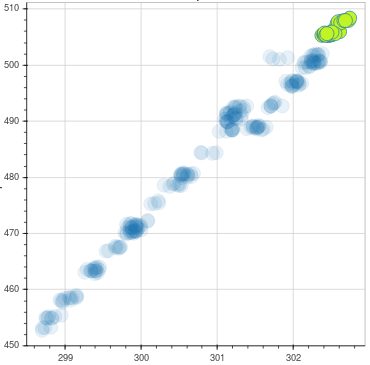
\includegraphics[width=0.9\linewidth]{figures/unsupervised/features/assm-16/u235-fiss/mean-pcm/mgxs-3}
  \caption{}
  \label{fig:chap10-fiss-mean-pcm-mgxs-3}
\end{subfigure}
\caption[Clustering of U-235 fission MGXS fractional reactivities]{Scatter plots of the pin-wise U-235 fission (group 2 of 2) \ac{MGXS} means ($x$) and fractional reactivities ($y$) for the 1.6\% enriched fuel assembly.}
\label{fig:chap10-mean-pcm}
\end{figure}

\clearpage

\begin{figure}[h!]
\centering
\begin{subfigure}{0.45\textwidth}
  \centering
  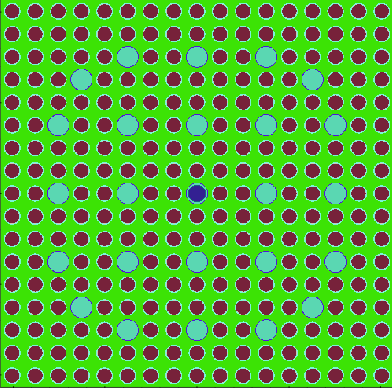
\includegraphics[width=0.9\linewidth]{figures/unsupervised/features/assm-16/geometry}
  \caption{}
  \label{fig:chap10-capt-mean-pcm-geom}
\end{subfigure}%
\begin{subfigure}{0.45\textwidth}
  \centering
  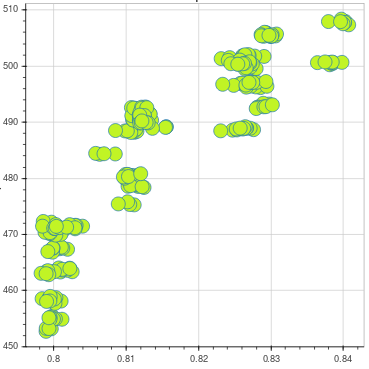
\includegraphics[width=0.9\linewidth]{figures/unsupervised/features/assm-16/u238-capt/mean-pcm/mgxs}
  \caption{}
  \label{fig:chap10-capt-mean-pcm-mgxs}
\end{subfigure}
\begin{subfigure}{0.45\textwidth}
  \centering
  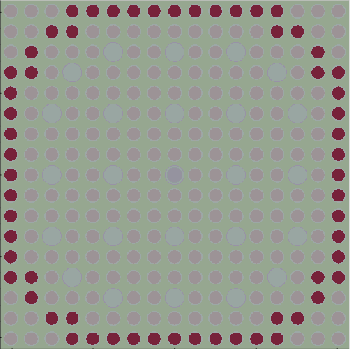
\includegraphics[width=0.9\linewidth]{figures/unsupervised/features/assm-16/u238-capt/mean-pcm/geometry-2}
  \caption{}
  \label{fig:chap10-capt-mean-pcm-geom-2}
\end{subfigure}%
\begin{subfigure}{0.45\textwidth}
  \centering
  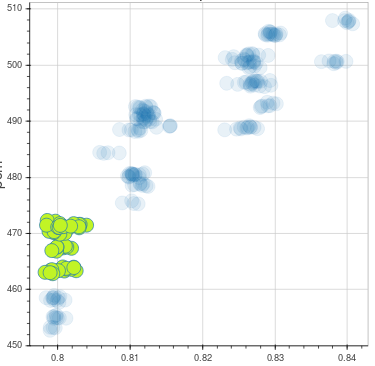
\includegraphics[width=0.9\linewidth]{figures/unsupervised/features/assm-16/u238-capt/mean-pcm/mgxs-2}
  \caption{}
  \label{fig:chap10-capt-mean-pcm-mgxs-2}
\end{subfigure}
\begin{subfigure}{0.45\textwidth}
  \centering
  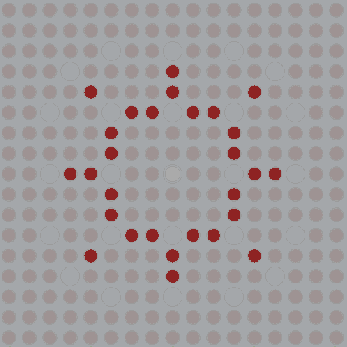
\includegraphics[width=0.9\linewidth]{figures/unsupervised/features/assm-16/u238-capt/mean-pcm/geometry-3}
  \caption{}
  \label{fig:chap10-capt-mean-pcm-geom-3}
\end{subfigure}%
\begin{subfigure}{0.45\textwidth}
  \centering
  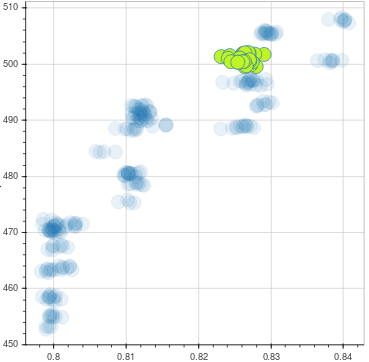
\includegraphics[width=0.9\linewidth]{figures/unsupervised/features/assm-16/u238-capt/mean-pcm/mgxs-3}
  \caption{}
  \label{fig:chap10-capt-mean-pcm-mgxs-3}
\end{subfigure}
\caption[Clustering of U-238 capture MGXS fractional reactivities]{Scatter plots of the pin-wise U-238 capture (group 1 of 2) \ac{MGXS} means ($x$) and fractional reactivities ($y$) for the 1.6\% enriched fuel assembly.}
\label{fig:chap10-mean-pcm}
\end{figure}

\clearpage


%%%%%%%%%%%%%%%%%%%%%%%%%%%
\subsection{Spectral Index}
\label{subsec:chap10-spec-index}

first paragraph: explain what it is
-divide each pin's nu-fission and absorption \ac{MGXS} 
-Eqn.~\ref{eqn:chap10-spec-index}
-explain what it indicates (differential moderation, adjacency to guide tubes, spectral hardening)
-note $i$ and $j$ may designate two difference nuclides
-note $\gamma$ is radiative capture - need to change this in theory section???

\begin{equation}
\label{eqn:chap10-spec-index-general}
\beta_{x,i,k,g} = \frac{\hat{\sigma}_{x,i,k,g}}{\hat{\sigma}_{f,k,g}^{235}}
\end{equation}

\begin{equation}
\label{eqn:chap10-spec-index-u238-capt}
\beta_{\gamma,k,g}^{238} = \frac{\hat{\sigma}_{\gamma,k,g}^{238}}{\hat{\sigma}_{f,k,g}^{235}}
\end{equation}

second paragraph: visualizations
-look at single fuel assembly with GUI
-three plots: full, two different clusters selected
-indicate which energy group and nuclide

\begin{figure}[h!]
\centering
\begin{subfigure}{0.42\textwidth}
  \centering
  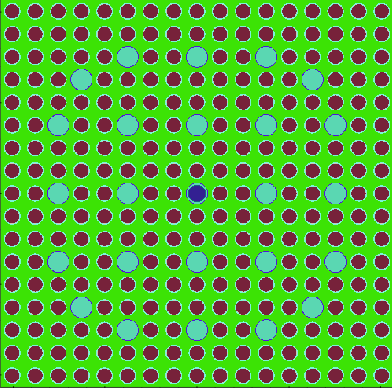
\includegraphics[width=0.9\linewidth]{figures/unsupervised/features/assm-16/geometry}
  \caption{}
  \label{fig:chap10-fiss-mean-spect-ind-geom}
\end{subfigure}%
\begin{subfigure}{0.42\textwidth}
  \centering
  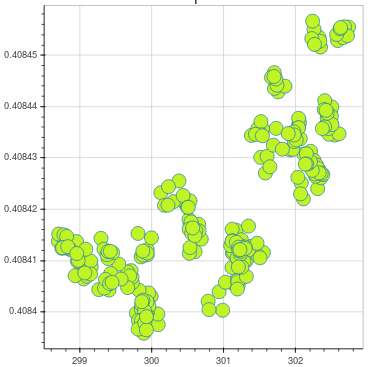
\includegraphics[width=0.9\linewidth]{figures/unsupervised/features/assm-16/u235-fiss/mean-spect-ind/mgxs}
  \caption{}
  \label{fig:chap10-fiss-mean-spect-ind-mgxs}
\end{subfigure}
\begin{subfigure}{0.42\textwidth}
  \centering
  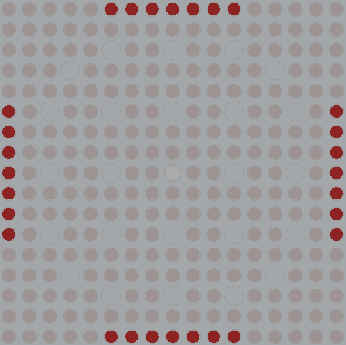
\includegraphics[width=0.9\linewidth]{figures/unsupervised/features/assm-16/u235-fiss/mean-spect-ind/geometry-2}
  \caption{}
  \label{fig:chap10-fiss-mean-spect-ind-geom-2}
\end{subfigure}%
\begin{subfigure}{0.42\textwidth}
  \centering
  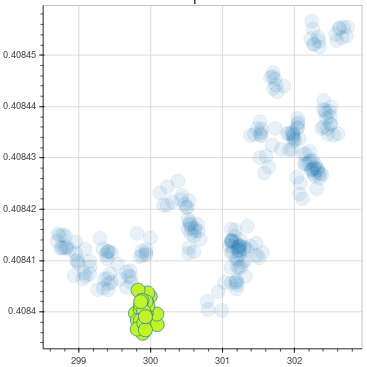
\includegraphics[width=0.9\linewidth]{figures/unsupervised/features/assm-16/u235-fiss/mean-spect-ind/mgxs-2}
  \caption{}
  \label{fig:chap10-fiss-mean-spect-ind-mgxs-2}
\end{subfigure}
\begin{subfigure}{0.42\textwidth}
  \centering
  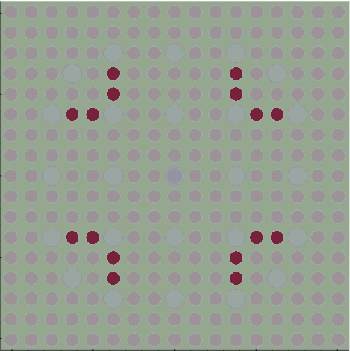
\includegraphics[width=0.9\linewidth]{figures/unsupervised/features/assm-16/u235-fiss/mean-spect-ind/geometry-3}
  \caption{}
  \label{fig:chap10-fiss-mean-spect-ind-geom-3}
\end{subfigure}%
\begin{subfigure}{0.42\textwidth}
  \centering
  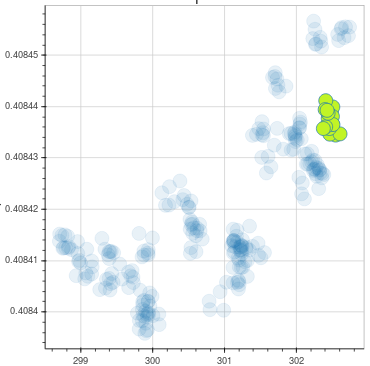
\includegraphics[width=0.9\linewidth]{figures/unsupervised/features/assm-16/u235-fiss/mean-spect-ind/mgxs-3}
  \caption{}
  \label{fig:chap10-fiss-mean-spect-ind-mgxs-3}
\end{subfigure}
\caption[Clustering of U-235 fission MGXS spectral indices]{Scatter plots of the pin-wise U-235 fission (group 2 of 2) \ac{MGXS} means ($x$) and spectral indices ($y$) for the 1.6\% enriched fuel assembly.}
\label{fig:chap10-mean-spect-ind}
\end{figure}

\clearpage

\begin{figure}[h!]
\centering
\begin{subfigure}{0.42\textwidth}
  \centering
  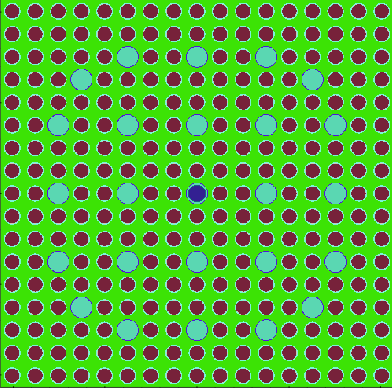
\includegraphics[width=0.9\linewidth]{figures/unsupervised/features/assm-16/geometry}
  \caption{}
  \label{fig:chap10-capt-mean-spect-ind-geom}
\end{subfigure}%
\begin{subfigure}{0.42\textwidth}
  \centering
  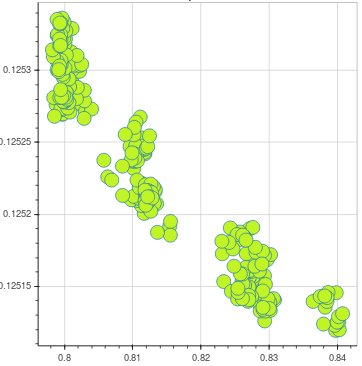
\includegraphics[width=0.9\linewidth]{figures/unsupervised/features/assm-16/u238-capt/mean-spect-ind/mgxs}
  \caption{}
  \label{fig:chap10-capt-mean-spect-ind-mgxs}
\end{subfigure}
\begin{subfigure}{0.42\textwidth}
  \centering
  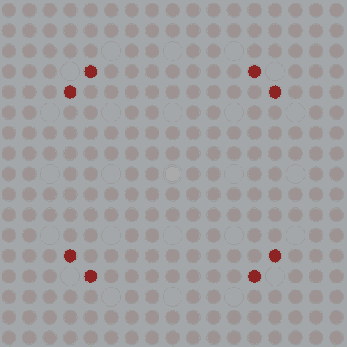
\includegraphics[width=0.9\linewidth]{figures/unsupervised/features/assm-16/u238-capt/mean-spect-ind/geometry-2}
  \caption{}
  \label{fig:chap10-capt-mean-spect-ind-geom-2}
\end{subfigure}%
\begin{subfigure}{0.42\textwidth}
  \centering
  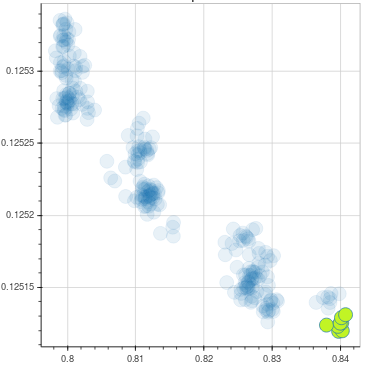
\includegraphics[width=0.9\linewidth]{figures/unsupervised/features/assm-16/u238-capt/mean-spect-ind/mgxs-2}
  \caption{}
  \label{fig:chap10-capt-mean-spect-ind-mgxs-2}
\end{subfigure}
\begin{subfigure}{0.42\textwidth}
  \centering
  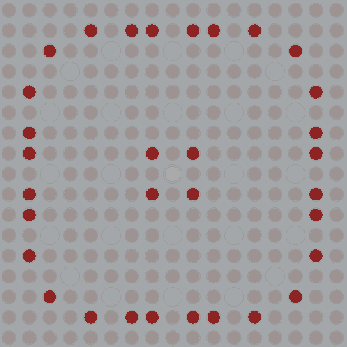
\includegraphics[width=0.9\linewidth]{figures/unsupervised/features/assm-16/u238-capt/mean-spect-ind/geometry-3}
  \caption{}
  \label{fig:chap10-capt-mean-spect-ind-geom-3}
\end{subfigure}%
\begin{subfigure}{0.42\textwidth}
  \centering
  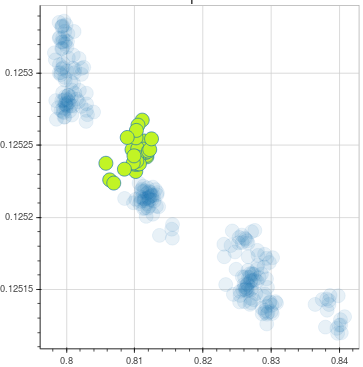
\includegraphics[width=0.9\linewidth]{figures/unsupervised/features/assm-16/u238-capt/mean-spect-ind/mgxs-3}
  \caption{}
  \label{fig:chap10-capt-mean-spect-ind-mgxs-3}
\end{subfigure}
\caption[Clustering of U-238 capture MGXS spectral indices]{Scatter plots of the pin-wise U-238 capture (group 1 of 2) \ac{MGXS} means ($x$) and spectral indices ($y$) for the 1.6\% enriched fuel assembly.}
\label{fig:chap10-mean-spect-ind}
\end{figure}

\clearpage

%%%%%%%%%%%%%%%%%%%%%%%%%%%%%
\subsection{Nuclide Fraction}
\label{subsec:chap10-nuclide-frac}

first paragraph: explain what it is
-divide pin-wise micro \ac{MGXS} for each nuclide/reaction/group by the corresponding total \ac{MGXS} for that nuclide/reaction/group trio
-Eqn.~\ref{eqn:chap10- nuclide-frac}
-explain what it indicates...???
-note $t$ designates the total collision reaction type

\begin{equation}
\label{eqn:chap10-nuclide-frac}
\tau_{x,i,k,g} = \frac{\hat{\sigma}_{x,i,k,g}}{\hat{\sigma}_{t,i,k,g}}
\end{equation}

second paragraph: visualizations
-look at single fuel assembly with GUI
-three plots: full, two different clusters selected
-indicate which energy group, nuclide, and reaction type

\begin{figure}[h!]
\centering
\begin{subfigure}{0.42\textwidth}
  \centering
  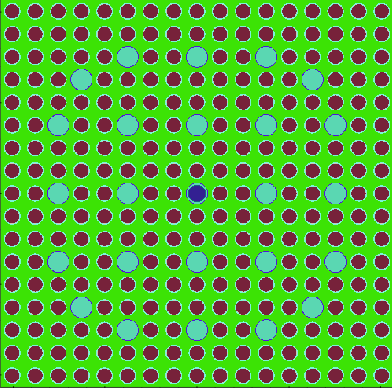
\includegraphics[width=0.9\linewidth]{figures/unsupervised/features/assm-16/geometry}
  \caption{}
  \label{fig:chap10-fiss-mean-nuc-frac-geom}
\end{subfigure}%
\begin{subfigure}{0.42\textwidth}
  \centering
  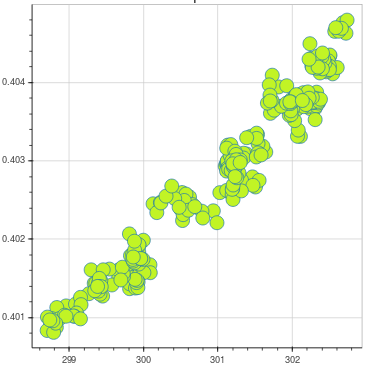
\includegraphics[width=0.9\linewidth]{figures/unsupervised/features/assm-16/u235-fiss/mean-nuc-frac/mgxs}
  \caption{}
  \label{fig:chap10-fiss-mean-nuc-frac-mgxs}
\end{subfigure}
\begin{subfigure}{0.42\textwidth}
  \centering
  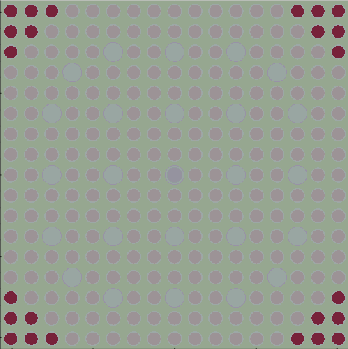
\includegraphics[width=0.9\linewidth]{figures/unsupervised/features/assm-16/u235-fiss/mean-nuc-frac/geometry-2}
  \caption{}
  \label{fig:chap10-fiss-mean-nuc-frac-geom-2}
\end{subfigure}%
\begin{subfigure}{0.42\textwidth}
  \centering
  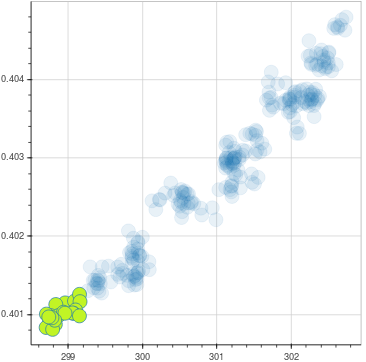
\includegraphics[width=0.9\linewidth]{figures/unsupervised/features/assm-16/u235-fiss/mean-nuc-frac/mgxs-2}
  \caption{}
  \label{fig:chap10-fiss-mean-nuc-frac-mgxs-2}
\end{subfigure}
\begin{subfigure}{0.42\textwidth}
  \centering
  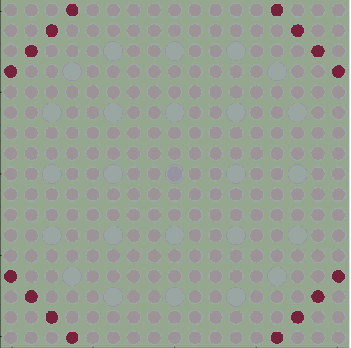
\includegraphics[width=0.9\linewidth]{figures/unsupervised/features/assm-16/u235-fiss/mean-nuc-frac/geometry-3}
  \caption{}
  \label{fig:chap10-fiss-mean-nuc-frac-geom-3}
\end{subfigure}%
\begin{subfigure}{0.42\textwidth}
  \centering
  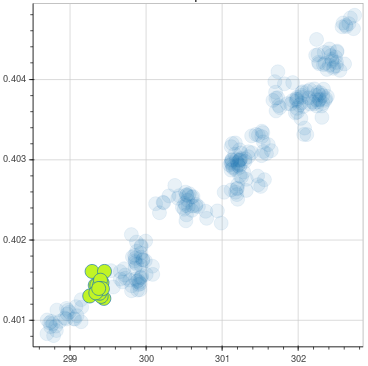
\includegraphics[width=0.9\linewidth]{figures/unsupervised/features/assm-16/u235-fiss/mean-nuc-frac/mgxs-3}
  \caption{}
  \label{fig:chap10-fiss-mean-nuc-frac-mgxs-3}
\end{subfigure}
\caption[Clustering of U-235 fission MGXS nuclide fractions]{Scatter plots of the pin-wise U-235 fission (group 2 of 2) \ac{MGXS} means ($x$) and nuclide fractions ($y$) for the 1.6\% enriched fuel assembly.}
\label{fig:chap10-mean-nuc-frac}
\end{figure}

\clearpage

\begin{figure}[h!]
\centering
\begin{subfigure}{0.42\textwidth}
  \centering
  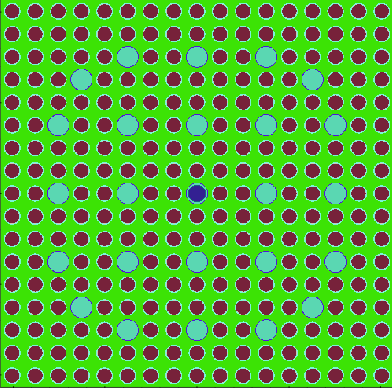
\includegraphics[width=0.9\linewidth]{figures/unsupervised/features/assm-16/geometry}
  \caption{}
  \label{fig:chap10-capt-mean-nuc-frac-geom}
\end{subfigure}%
\begin{subfigure}{0.42\textwidth}
  \centering
  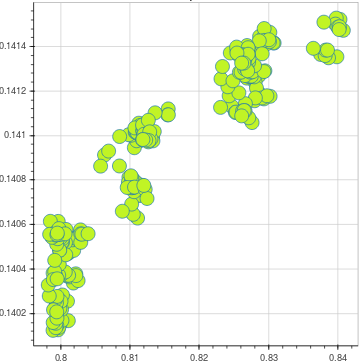
\includegraphics[width=0.9\linewidth]{figures/unsupervised/features/assm-16/u238-capt/mean-nuc-frac/mgxs}
  \caption{}
  \label{fig:chap10-capt-mean-nuc-frac-mgxs}
\end{subfigure}
\begin{subfigure}{0.42\textwidth}
  \centering
  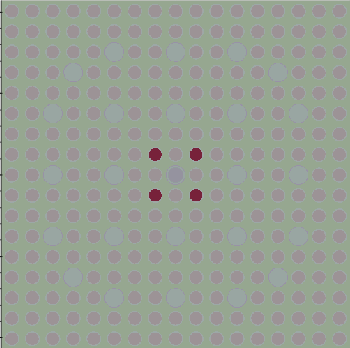
\includegraphics[width=0.9\linewidth]{figures/unsupervised/features/assm-16/u238-capt/mean-nuc-frac/geometry-2}
  \caption{}
  \label{fig:chap10-capt-mean-nuc-frac-geom-2}
\end{subfigure}%
\begin{subfigure}{0.42\textwidth}
  \centering
  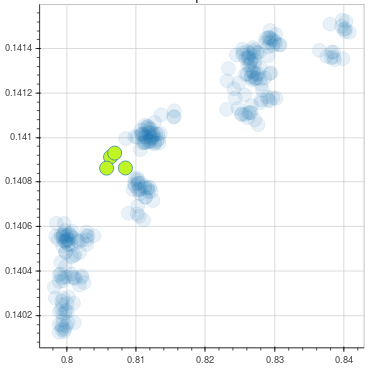
\includegraphics[width=0.9\linewidth]{figures/unsupervised/features/assm-16/u238-capt/mean-nuc-frac/mgxs-2}
  \caption{}
  \label{fig:chap10-capt-mean-nuc-frac-mgxs-2}
\end{subfigure}
\begin{subfigure}{0.42\textwidth}
  \centering
  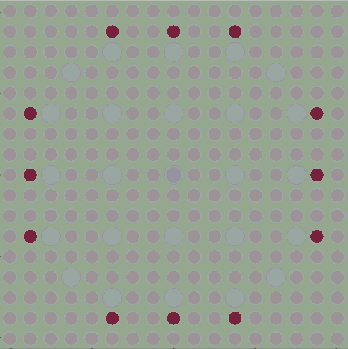
\includegraphics[width=0.9\linewidth]{figures/unsupervised/features/assm-16/u238-capt/mean-nuc-frac/geometry-3}
  \caption{}
  \label{fig:chap10-capt-mean-nuc-frac-geom-3}
\end{subfigure}%
\begin{subfigure}{0.42\textwidth}
  \centering
  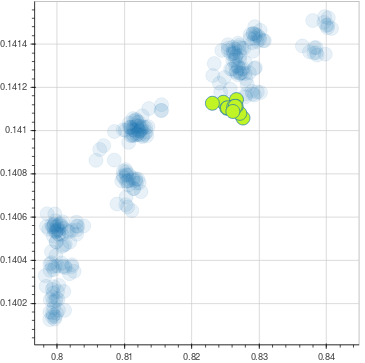
\includegraphics[width=0.9\linewidth]{figures/unsupervised/features/assm-16/u238-capt/mean-nuc-frac/mgxs-3}
  \caption{}
  \label{fig:chap10-capt-mean-nuc-frac-mgxs-3}
\end{subfigure}
\caption[Clustering of U-238 capture MGXS nuclide fractions]{Scatter plots of the pin-wise U-238 capture (group 1 of 2) \ac{MGXS} means ($x$) and nuclide fractions ($y$) for the 1.6\% enriched fuel assembly.}
\label{fig:chap10-mean-nuc-frac}
\end{figure}

\clearpage

%%%%%%%%%%%%%%%%%%%%%%%%%%%
\subsection{Total Fraction}
\label{subsec:chap10-tot-frac}

first paragraph: explain what it is
-divide pin-wise micro \ac{MGXS} for each nuclide/reaction/group by the corresponding total \ac{MGXS} for that nuclide/reaction/group trio
-Eqn.~\ref{eqn:chap10-tot-frac}
-explain what it indicates...???
-note that $I$ designates the total number of nuclides in a fuel pin

\begin{equation}
\label{eqn:chap10-tot-frac}
\omega_{x,i,k,g} = \frac{\hat{\sigma}_{x,i,k,g}}{\displaystyle\sum\limits_{i=1}^{I}\hat{\sigma}_{t,i,k,g}}
\end{equation}

second paragraph: visualizations
-look at single fuel assembly with GUI
-three plots: full, two different clusters selected
-indicate which energy group, nuclide, and reaction type

%%%%%%%%%%%%%%%%%%%%%%%%%%%%%%%%%%%%%%%%%%%%%%%%%%%%%%%%%%%%%%%%%%%%%%%%%%%%%%%
\section{Target Selection}
\label{sec:chap10-target-select}

%%%%%%%%%%%%%%%%%%%%%%%%%%%%%%%%%%%%%%%%%%%%%%%%%%%%%%%%%%%%%%%%%%%%%%%%%%%%%%%
\section{Feature Transformation}
\label{sec:chap10-feature-transform}

first paragraph: what is goal???
-curse of dimensionality - dimensionality reduction
-transform number of features to find new ones with more descriptive power than original set
  -new features may be more easily ordered than original ones
    -allowing for easier feature selection (Sec.~\ref{sec:chap10-litmus})
-can account for correlations between features
  -rather than treating each features independent

%%%%%%%%%%%%%%%%%%%%%%%%%%%%%%%%%%
\subsection{Feature Decomposition}
\label{subsec:chap10-feature-transform-decomp}

%%%%%%%%%%%%%%%%%%%%%%%%%%%%%%%%%%%%%%%%%
\subsection{Principal Component Analysis}
\label{subsec:chap10-feature-transform-pca}

%%%%%%%%%%%%%%%%%%%%%%%%%%%%%%%%%%%%%%%%%%%
\subsection{Independent Component Analysis}
\label{subsec:chap10-feature-transform-ica}

%%%%%%%%%%%%%%%%%%%%%%%%%%%%%%%%%%%%%%%%%
\subsection{Feature -- Target Regression}
\label{subsec:chap10-feature-transform-regression}


%%%%%%%%%%%%%%%%%%%%%%%%%%%%%%%%%%%%%%%%%%%%%%%%%%%%%%%%%%%%%%%%%%%%%%%%%%%%%%%
\section{Feature Selection}
\label{sec:chap10-litmus}

-dimensionality reduction

%%%%%%%%%%%%%%%%%%%%%%%%%%%%%%%%%%%%%%%%%%%%%%%%%%%%%%%%%%%%%%%%%%%%%%%%%%%%%%%
\section{Litmus Tests}
\label{sec:chap10-litmus}

first paragraph: what are ``litmust tests''?
-which \ac{MGXS} need to be clustered
  -which nuclides
  -which reaction type
  -which energy group

-first choose a reaction type for a nuclide, energy group
-then run litmus tests to determine whether to cluster it

-note that results in following chapter may not make full use of litmus tests
  -instead, user will indicate wish to cluster individual MGXS like U-238 capture

%%%%%%%%%%%%%%%%%%%%%%%%%%%%%
\subsection{Nuclide Fraction}
\label{subsec:chap10-litmus-nuc-frac}

-used to choose reaction type
-threshold on $\tau_{x,i,k,g}$
-only choose reaction's which contribute at least some amount towards the total cross section
  -assumes that reaction with little contribution are not important to cluster anyway
  -but may mistakenly make approx that MGXS with small magnitudes don't disproportionately reflect self-shielding effects
    -but this is a good assumption since larger MGXS will have smaller uncertainties anyway

%%%%%%%%%%%%%%%%%%%%%%%%%%%%%%%%%%%%%%%%%%
\subsection{Nuclide Fraction Thresholding}
\label{subsec:chap10-litmus-nuc-frac}

-used to choose reaction type
-threshold on the population variance divide by the population mean

%%%%%%%%%%%%%%%%%%%%%%%%%%%%%%%%%%%%%%%%
\subsection{Total Fraction Thresholding}
\label{subsec:chap10-litmus-tot-frac}

-used to determine whether to cluster MGXS for a particular nuclide, group, rxn type
-threshold on $\omega_{x,i,k,g}$
  -only cluster if the MGXS makes up a substantial fraction of the MGXS for all nuclides
  -otherwise, self-shielding of the nuclide won't matter anyway
  -this must be of the macro not the micro MGXS btw!!!

%%%%%%%%%%%%%%%%%%%%%%%%%%%%
\subsection{Normality Tests}
\label{subsec:chap10-litmus-normality}

-used to determine whether to cluster MGXS for a particular nuclide, group, rxn type
-look at $p$-value for Shapiro-Wilks tests of normality
-don't cluster data that may have come from a normal distribution!
-if the $p$-value is below a threshold, then data may be rejected as non-normal and may be good candidate for clustering



%%%%%%%%%%%%%%%%%%%%%%%%%%%%%%%%%%%%%%%%%%%%%%%%%%%%%%%%%%%%%%%%%%%%%%%%%%%%%%%
\section{Clustering Algorithms}
\label{subsec:chap10-clustering}

-very brief overview
-refer to literature for more info
-used canned algorithms in scikit-learn \texttt{sklearn.cluster}
-while there are many, many algorithms out there, only a few selected for discussion here
  -one concern is scalability to large number of samples

%%%%%%%%%%%%%%%%%%%%%%%%%%%%%%%%%
\subsection{$k$-Means Clustering}
\label{subsec:chap10-kmeans}

-introduce scheme
-algorithmic
-initialization
-model selection

%%%%%%%%%%%%%%%%%%%%%%%%%%%%%%%%%%%%
\subsection{Hierarchical Clustering}
\label{subsec:chap10-agglomerative}

-introduce scheme
-algorithmic
-initialization
-model selection

%%%%%%%%%%%%%%%%%%%%%%%%%%%%
\subsection{DBSCAN}
\label{subsec:chap10-dbscan}

-introduce scheme
-algorithmic
-initialization
-model selection

%%%%%%%%%%%%%%%%%%%%%%%%%%%%%%%%%
\section{Gaussian Mixture Models}
\label{sec:chap10-gmms}

-introduce scheme
-algorithmic
-initialization
-intro fact that it is not scalable - not evaluated here
-mention dirichlet process mixture models
-model selection criteria are nice
-model selection

%%%%%%%%%%%%%%%%%%%%%%%%%%%%%%%%%%%%%%%%%%%%%%%%%%%%%%%%%%%%%%%%%%%%%%%%%%%%%%%
\section{Clustered Geometries}
\label{sec:chap10-geometries}

-agglomerative clustering was used to generate the figures
-which nuclide, group, reaction was used for pinch clustering???

\begin{figure}[h!]
\centering
\begin{subfigure}{0.48\textwidth}
  \centering
  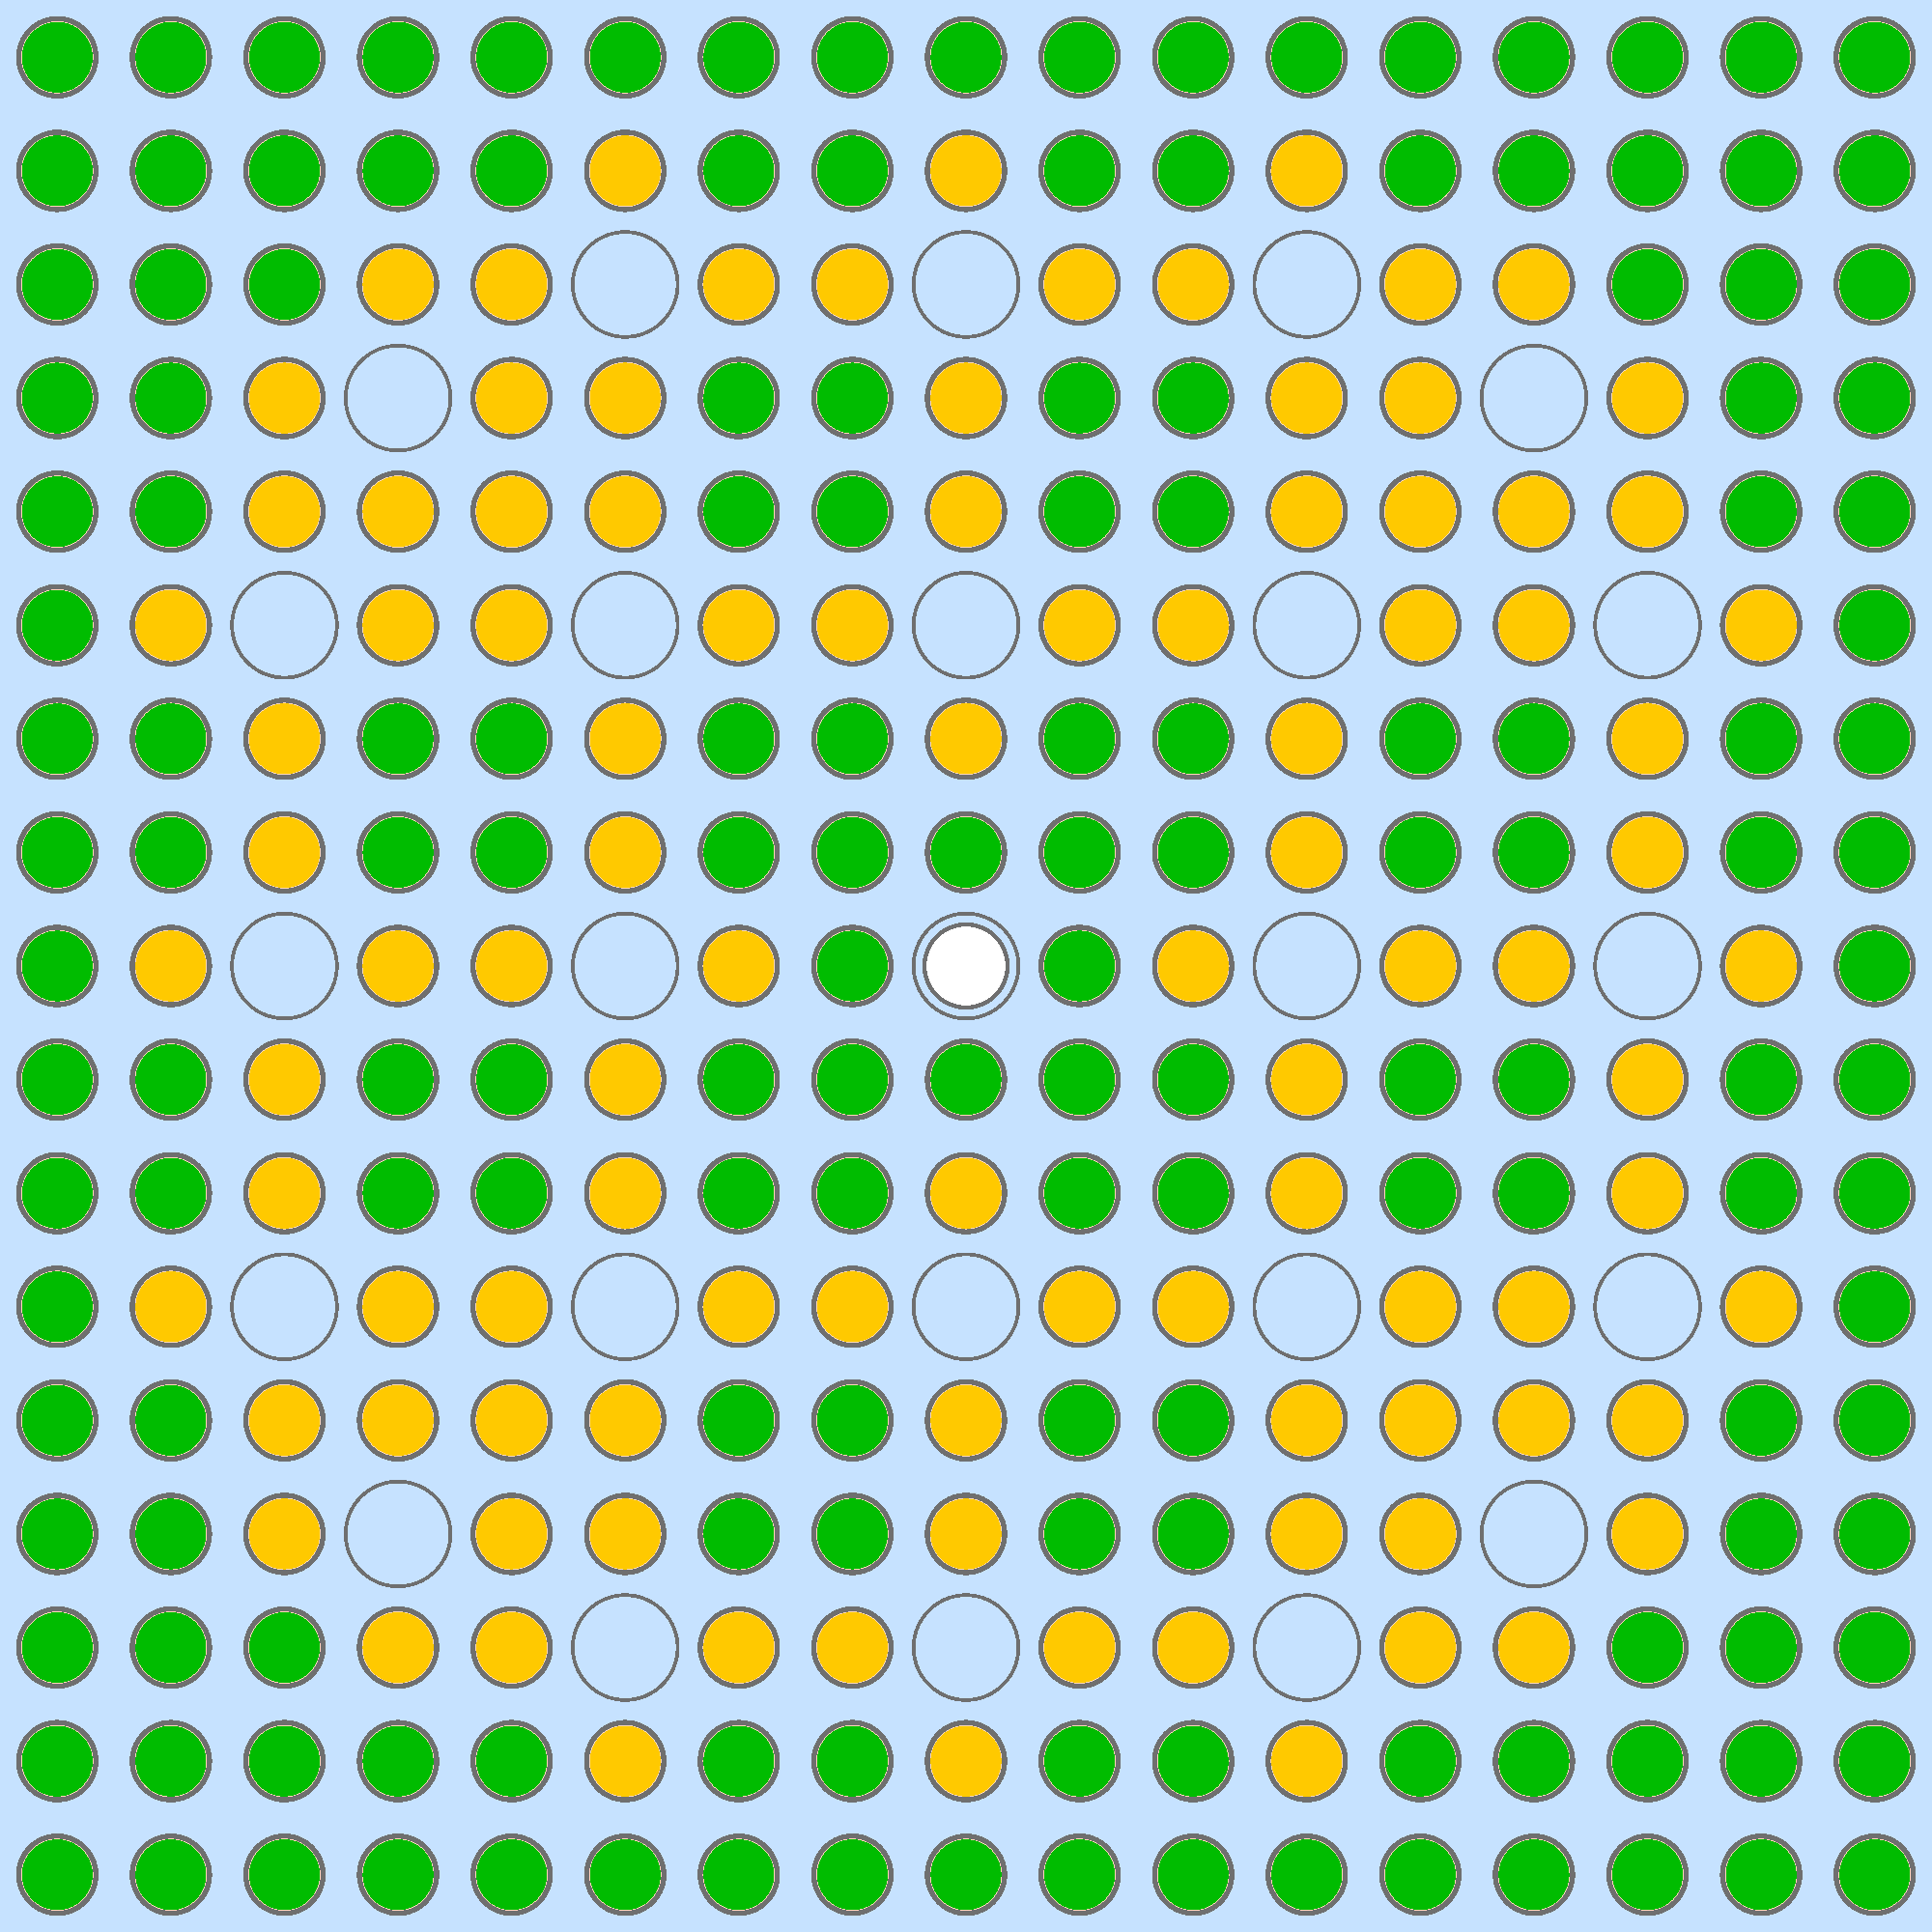
\includegraphics[width=0.9\linewidth]{figures/unsupervised/geometries/with-features/2-clusters/pinch/assm-16}
  \caption{}
  \label{fig:chap10-assm-16-pinch-2}
\end{subfigure}%
\begin{subfigure}{0.48\textwidth}
  \centering
  \includegraphics[width=0.9\linewidth]{figures/unsupervised/geometries/with-features/2-clusters/combined/assm-16}
  \caption{}
  \label{fig:chap10-assm-16-combined-2}
\end{subfigure}
\begin{subfigure}{0.48\textwidth}
  \centering
  \includegraphics[width=0.9\linewidth]{figures/unsupervised/geometries/with-features/4-clusters/pinch/assm-16}
  \caption{}
  \label{fig:chap10-assm-16-pinch-4}
\end{subfigure}%
\begin{subfigure}{0.48\textwidth}
  \centering
  \includegraphics[width=0.9\linewidth]{figures/unsupervised/geometries/with-features/4-clusters/combined/assm-16}
  \caption{}
  \label{fig:chap10-assm-16-combined-4}
\end{subfigure}
\begin{subfigure}{0.48\textwidth}
  \centering
  \includegraphics[width=0.9\linewidth]{figures/unsupervised/geometries/with-features/8-clusters/pinch/assm-16}
  \caption{}
  \label{fig:chap10-assm-16-pinch-8}
\end{subfigure}%
\begin{subfigure}{0.48\textwidth}
  \centering
  \includegraphics[width=0.9\linewidth]{figures/unsupervised/geometries/with-features/8-clusters/combined/assm-16}
  \caption{}
  \label{fig:chap10-assm-16-combined-8}
\end{subfigure}
\caption[Materials for the 1.6\% fuel assembly with clustering homogenization]{Materials for the 1.6\% enriched fuel assembly with clustering homogenization. The materials for 2, 4, and 8 clusters are illustrated in (a), (c) and (e) for pinch clustering, and in (b), (d) and (f) for combined clustering, respectively.}
\label{fig:chap10-assm-16-geometries}
\end{figure}

\clearpage

\begin{figure}[h!]
\centering
\begin{subfigure}{0.48\textwidth}
  \centering
  \includegraphics[width=0.9\linewidth]{figures/unsupervised/geometries/with-features/2-clusters/pinch/assm-31-20BPs}
  \caption{}
  \label{fig:chap10-assm-31-20BPs-pinch-2}
\end{subfigure}%
\begin{subfigure}{0.48\textwidth}
  \centering
  \includegraphics[width=0.9\linewidth]{figures/unsupervised/geometries/with-features/2-clusters/combined/assm-31-20BPs}
  \caption{}
  \label{fig:chap10-assm-31-20BPs-combined-2}
\end{subfigure}
\begin{subfigure}{0.48\textwidth}
  \centering
  \includegraphics[width=0.9\linewidth]{figures/unsupervised/geometries/with-features/4-clusters/pinch/assm-31-20BPs}
  \caption{}
  \label{fig:chap10-assm-31-20BPs-pinch-4}
\end{subfigure}%
\begin{subfigure}{0.48\textwidth}
  \centering
  \includegraphics[width=0.9\linewidth]{figures/unsupervised/geometries/with-features/4-clusters/combined/assm-31-20BPs}
  \caption{}
  \label{fig:chap10-assm-31-20BPs-combined-4}
\end{subfigure}
\begin{subfigure}{0.48\textwidth}
  \centering
  \includegraphics[width=0.9\linewidth]{figures/unsupervised/geometries/with-features/8-clusters/pinch/assm-31-20BPs}
  \caption{}
  \label{fig:chap10-assm-31-20BPs-pinch-8}
\end{subfigure}%
\begin{subfigure}{0.48\textwidth}
  \centering
  \includegraphics[width=0.9\linewidth]{figures/unsupervised/geometries/with-features/8-clusters/combined/assm-31-20BPs}
  \caption{}
  \label{fig:chap10-assm-31-20BPs-combined-8}
\end{subfigure}
\caption[Materials for the 3.1\% fuel assembly with clustering homogenization]{Materials for the 3.1\% enriched fuel assembly with 20 \acp{BP} with clustering homogenization. The materials for 2, 4, and 8 clusters are illustrated in (a), (c) and (e) for pinch clustering, and in (b), (d) and (f) for combined clustering, respectively.}
\label{fig:chap10-assm-31-20BPs-geometries}
\end{figure}

\clearpage

\begin{figure}[h!]
\centering
\begin{subfigure}{0.48\textwidth}
  \centering
  \includegraphics[width=0.9\linewidth]{figures/unsupervised/geometries/with-features/2-clusters/pinch/2x2}
  \caption{}
  \label{fig:chap10-2x2-pinch-2}
\end{subfigure}%
\begin{subfigure}{0.48\textwidth}
  \centering
  \includegraphics[width=0.9\linewidth]{figures/unsupervised/geometries/with-features/2-clusters/combined/2x2}
  \caption{}
  \label{fig:chap10-2x2-combined-2}
\end{subfigure}
\begin{subfigure}{0.48\textwidth}
  \centering
  \includegraphics[width=0.9\linewidth]{figures/unsupervised/geometries/with-features/4-clusters/pinch/2x2}
  \caption{}
  \label{fig:chap10-2x2-pinch-4}
\end{subfigure}%
\begin{subfigure}{0.48\textwidth}
  \centering
  \includegraphics[width=0.9\linewidth]{figures/unsupervised/geometries/with-features/4-clusters/combined/2x2}
  \caption{}
  \label{fig:chap10-assm-2x2-combined-4}
\end{subfigure}
\begin{subfigure}{0.48\textwidth}
  \centering
  \includegraphics[width=0.9\linewidth]{figures/unsupervised/geometries/with-features/8-clusters/pinch/2x2}
  \caption{}
  \label{fig:chap10-assm-2x2-pinch-8}
\end{subfigure}%
\begin{subfigure}{0.48\textwidth}
  \centering
  \includegraphics[width=0.9\linewidth]{figures/unsupervised/geometries/with-features/8-clusters/combined/2x2}
  \caption{}
  \label{fig:chap10-assm-2x2-combined-8}
\end{subfigure}
\caption[Materials for the 2$\times$2 periodic colorset with clustering homogenization]{Materials for the 2$\times$2 periodic colorset with clustering homogenization. The materials for 2, 4, and 8 clusters are illustrated in (a), (c) and (e) for pinch clustering, and in (b), (d) and (f) for combined clustering, respectively.}
\label{fig:chap10-2x2-geometries}
\end{figure}

\clearpage

\begin{figure}[h!]
\centering
\begin{subfigure}{0.48\textwidth}
  \centering
  \includegraphics[width=0.9\linewidth]{figures/unsupervised/geometries/with-features/2-clusters/pinch/reflector}
  \caption{}
  \label{fig:chap10-reflector-pinch-2}
\end{subfigure}%
\begin{subfigure}{0.48\textwidth}
  \centering
  \includegraphics[width=0.9\linewidth]{figures/unsupervised/geometries/with-features/2-clusters/combined/reflector}
  \caption{}
  \label{fig:chap10-reflector-combined-2}
\end{subfigure}
\begin{subfigure}{0.48\textwidth}
  \centering
  \includegraphics[width=0.9\linewidth]{figures/unsupervised/geometries/with-features/4-clusters/pinch/reflector}
  \caption{}
  \label{fig:chap10-reflector-pinch-4}
\end{subfigure}%
\begin{subfigure}{0.48\textwidth}
  \centering
  \includegraphics[width=0.9\linewidth]{figures/unsupervised/geometries/with-features/4-clusters/combined/reflector}
  \caption{}
  \label{fig:chap10-reflector-combined-4}
\end{subfigure}
\begin{subfigure}{0.48\textwidth}
  \centering
  \includegraphics[width=0.9\linewidth]{figures/unsupervised/geometries/with-features/8-clusters/pinch/reflector}
  \caption{}
  \label{fig:chap10-reflector-pinch-8}
\end{subfigure}%
\begin{subfigure}{0.48\textwidth}
  \centering
  \includegraphics[width=0.9\linewidth]{figures/unsupervised/geometries/with-features/8-clusters/combined/reflector}
  \caption{}
  \label{fig:chap10-reflector-combined-8}
\end{subfigure}
\caption[Materials for the 2$\times$2 colorset with reflector with clustering homogenization]{Materials for the 2$\times$ colorset with water reflector with clustering homogenization. The materials for 2, 4, and 8 clusters are illustrated in (a), (c) and (e) for pinch clustering, and in (b), (d) and (f) for combined clustering, respectively.}
\label{fig:chap10-reflector-geometries}
\end{figure}

\clearpage

\begin{figure}[h!]
\centering
\begin{subfigure}{0.48\textwidth}
  \centering
  \includegraphics[width=0.9\linewidth]{figures/unsupervised/geometries/with-features/2-clusters/pinch/full-core}
  \caption{}
  \label{fig:chap10-full-core-pinch-2}
\end{subfigure}%
\begin{subfigure}{0.48\textwidth}
  \centering
  \includegraphics[width=0.9\linewidth]{figures/unsupervised/geometries/with-features/2-clusters/combined/full-core}
  \caption{}
  \label{fig:chap10-full-core-combined-2}
\end{subfigure}
\begin{subfigure}{0.48\textwidth}
  \centering
  \includegraphics[width=0.9\linewidth]{figures/unsupervised/geometries/with-features/4-clusters/pinch/full-core}
  \caption{}
  \label{fig:chap10-full-core-pinch-4}
\end{subfigure}%
\begin{subfigure}{0.48\textwidth}
  \centering
  \includegraphics[width=0.9\linewidth]{figures/unsupervised/geometries/with-features/4-clusters/combined/full-core}
  \caption{}
  \label{fig:chap10-full-core-combined-4}
\end{subfigure}
\begin{subfigure}{0.48\textwidth}
  \centering
  \includegraphics[width=0.9\linewidth]{figures/unsupervised/geometries/with-features/8-clusters/pinch/full-core}
  \caption{}
  \label{fig:chap10-full-core-pinch-8}
\end{subfigure}%
\begin{subfigure}{0.48\textwidth}
  \centering
  \includegraphics[width=0.9\linewidth]{figures/unsupervised/geometries/with-features/8-clusters/combined/full-core}
  \caption{}
  \label{fig:chap10-full-core-combined-8}
\end{subfigure}
\caption[Materials for BEAVRS with clustering homogenization (2 -- 8 clusters)]{Materials for the quarter core \ac{BEAVRS} model with clustering homogenization. The materials for 2, 4, and 8 clusters are illustrated in (a), (c) and (e) for pinch clustering, and in (b), (d) and (f) for combined clustering, respectively.}
\label{fig:chap10-full-core-geometries-8}
\end{figure}

\clearpage

\begin{figure}[h!]
\centering
\begin{subfigure}{0.48\textwidth}
  \centering
  \includegraphics[width=0.9\linewidth]{figures/unsupervised/geometries/with-features/16-clusters/pinch/full-core}
  \caption{}
  \label{fig:chap10-full-core-pinch-16}
\end{subfigure}%
\begin{subfigure}{0.48\textwidth}
  \centering
  \includegraphics[width=0.9\linewidth]{figures/unsupervised/geometries/with-features/16-clusters/combined/full-core}
  \caption{}
  \label{fig:chap10-full-core-combined-16}
\end{subfigure}
\begin{subfigure}{0.48\textwidth}
  \centering
  \includegraphics[width=0.9\linewidth]{figures/unsupervised/geometries/with-features/32-clusters/pinch/full-core}
  \caption{}
  \label{fig:chap10-full-core-pinch-32}
\end{subfigure}%
\begin{subfigure}{0.48\textwidth}
  \centering
  \includegraphics[width=0.9\linewidth]{figures/unsupervised/geometries/with-features/32-clusters/combined/full-core}
  \caption{}
  \label{fig:chap10-full-core-combined-32}
\end{subfigure}
\begin{subfigure}{0.48\textwidth}
  \centering
  \includegraphics[width=0.9\linewidth]{figures/unsupervised/geometries/with-features/64-clusters/pinch/full-core}
  \caption{}
  \label{fig:chap10-full-core-pinch-64}
\end{subfigure}%
\begin{subfigure}{0.48\textwidth}
  \centering
  \includegraphics[width=0.9\linewidth]{figures/unsupervised/geometries/with-features/64-clusters/combined/full-core}
  \caption{}
  \label{fig:chap10-full-core-combined-64}
\end{subfigure}
\caption[Materials for BEAVRS with clustering homogenization (16 -- 64 clusters)]{Materials for the quarter core \ac{BEAVRS} model with clustering homogenization. The materials for 16, 32, and 64 clusters are illustrated in (a), (c) and (e) for pinch clustering, and in (b), (d) and (f) for combined clustering, respectively.}
\label{fig:chap10-full-core-geometries-64}
\end{figure}

\clearpage

%%%%%%%%%%%%%%%%%%%%%%%%%%%%%%%%%%%%%%%%%%%%%%%%%%%%%%%%%%%%%%%%%%%%%%%%%%%%%%%
\section{Evaluating the Methodology}
\label{sec:chap10-cluster}

%%%%%%%%%%%%%%%%%%%%%%%%%%%%%%%
\subsection{Perfect Clustering}
\label{subsec:chap10-perfect-cluster}

%%%%%%%%%%%%%%%%%%%%%%%%%%%%%%%%
\subsection{Adaptive Clustering}
\label{subsec:chap10-adaptive-cluster}

\begin{itemize}[noitemsep]
  \item dataset restrictions
  \begin{itemize}[noitemsep]
    \item \textbf{``pinch'' clustering} - a \textit{single} nuclide/group/reaction triplet
    \item \textbf{``combined'' clustering} - one or more nuclide/group pairs \textit{together}
    \item \textbf{``local'' clustering} - one or more nuclide/group pairs \textit{separately}
  \end{itemize}
  \item clustering algorithms
  \begin{itemize}[noitemsep]
    \item discriminative clustering ($k$-Means++, Agglomerative, etc.)
    \item generative clustering (Gaussian Mixtures, Dirichlet Processes)
  \end{itemize}
  \item ``regression-informed'' clustering
  \begin{itemize}[noitemsep]
    \item use a regressor to predict ``smoothed'' of target variable(s)
    \begin{itemize}[noitemsep]
      \item decision tree regression
      \item ensemble (boosting, random forest) regression
      \item Gaussian Process regression
    \end{itemize}
    \item cluster predictions produced by regressor
    \item advantage is that objective function \textit{may} be more appropriate
  \end{itemize}
\end{itemize}